\documentclass[a4paper]{article}

\usepackage{tikz}
\usetikzlibrary{positioning, arrows.meta, shapes, calc, fit, backgrounds}
\usepackage{float}
\usepackage{geometry}
\geometry{margin=0.5cm, landscape}

\begin{document}

\title{System Overview: HYPOTHETICAL "Neuro-Symbolic Super Prosimos"}
\author{}
\date{}
\maketitle

\section{Hypothetical Architecture: Neuro-Symbolic Runtime Engine}

This diagram illustrates the "Dream Architecture": A Hybrid Engine that combines \textbf{Discrete Event Simulation (DES)} for resource management, \textbf{Deep Learning (LSTM)} for path prediction, and \textbf{Declarative Logic (LTL)} for rule enforcement at runtime.

\begin{figure}[H]
  \centering
  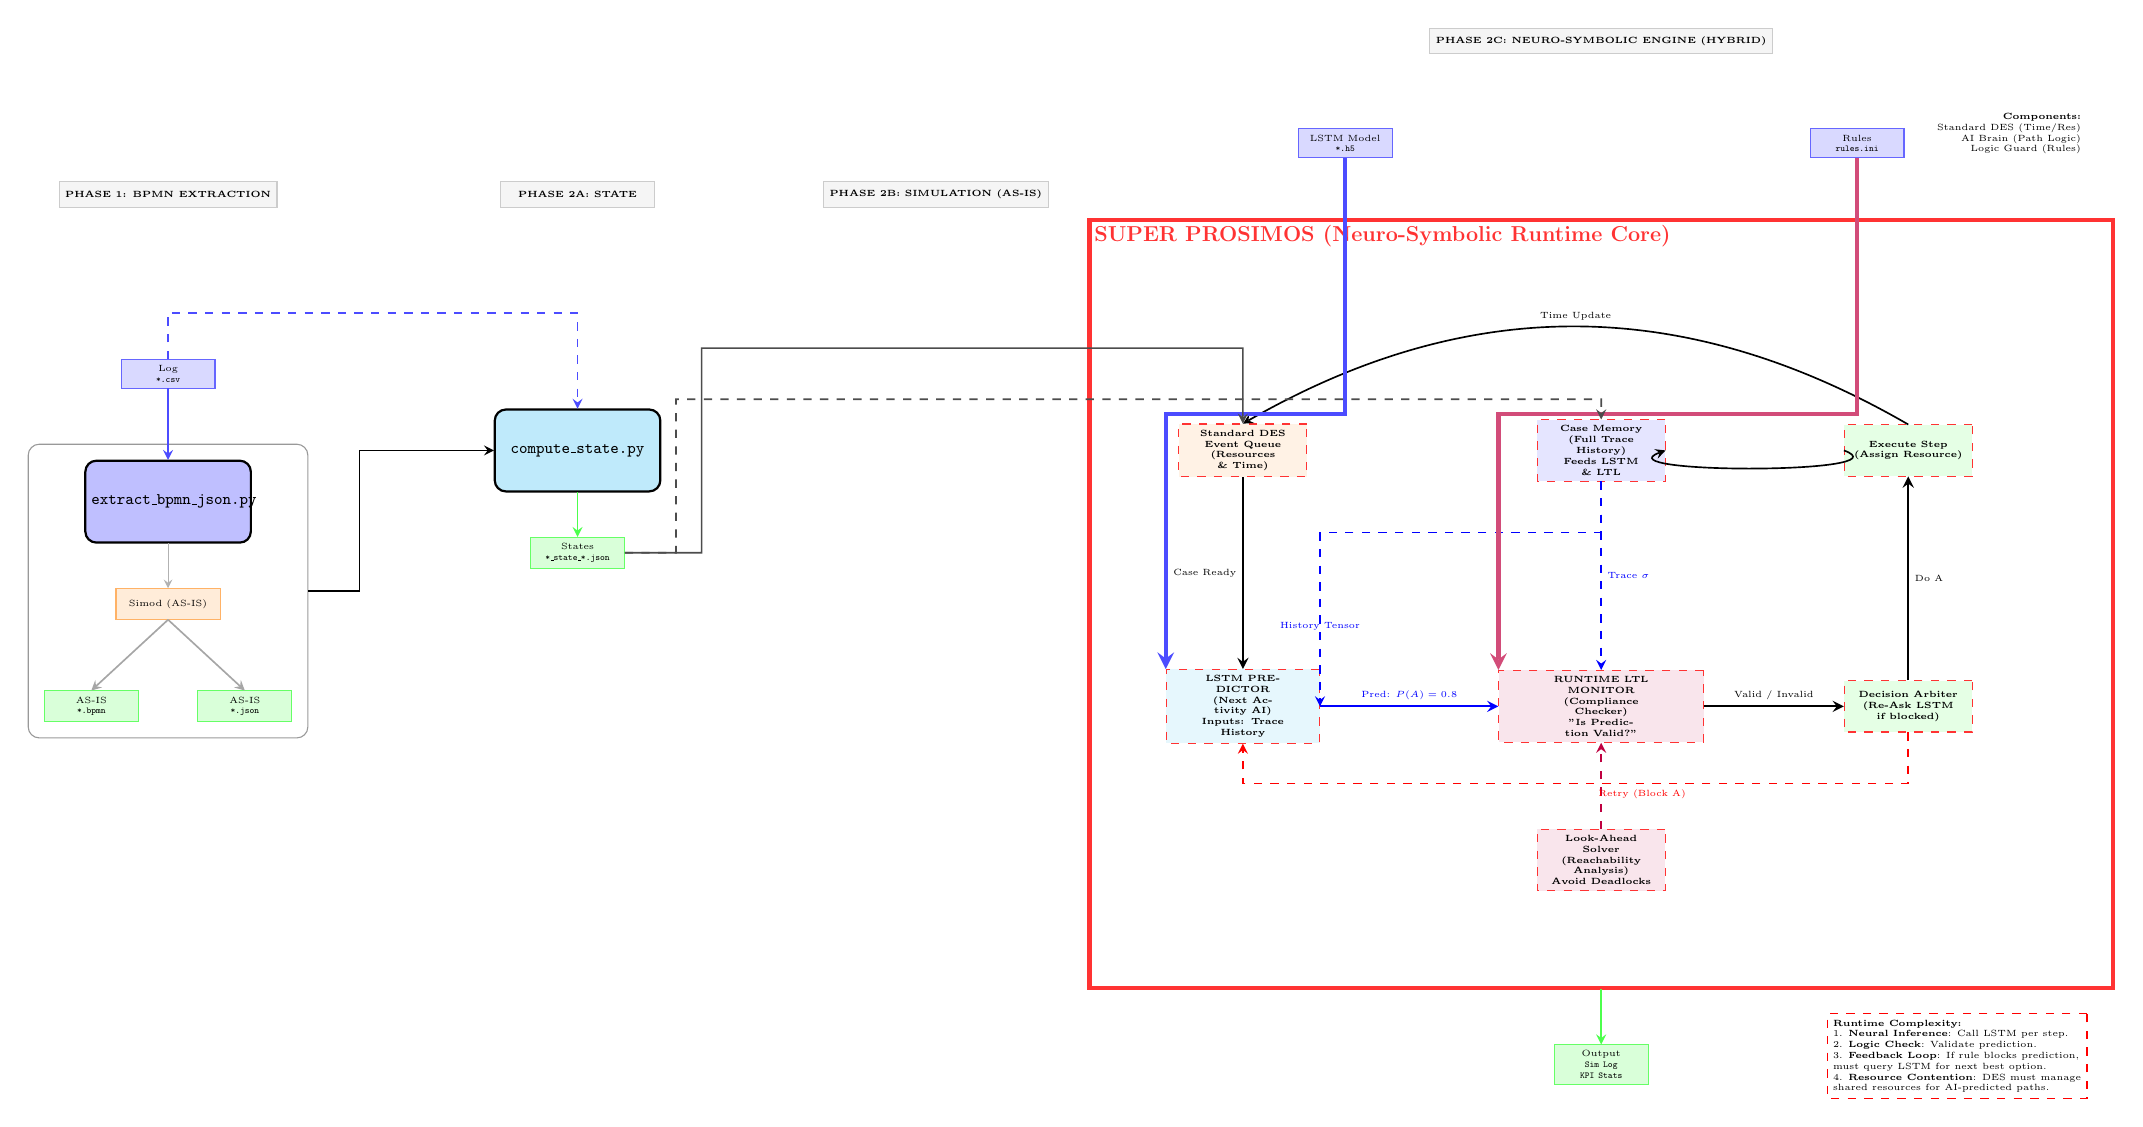
\begin{tikzpicture}[
    scale=0.65,
    transform shape,
    node distance=0.8cm and 1.5cm,
    script/.style={rectangle, rounded corners, draw=black, thick, 
                   minimum width=3.2cm, minimum height=1.6cm, 
                   text width=3cm, align=center, font=\small\bfseries},
    procstep/.style={rectangle, rounded corners, draw=black, fill=gray!10,
                 minimum width=2.5cm, minimum height=0.6cm,
                 text width=2.3cm, align=center, font=\tiny},
    input/.style={rectangle, draw=blue!60, fill=blue!15, 
                  minimum width=1.8cm, minimum height=0.5cm, 
                  text width=1.6cm, align=center, font=\tiny},
    output/.style={rectangle, draw=green!60, fill=green!15, 
                   minimum width=1.8cm, minimum height=0.5cm, 
                   text width=1.6cm, align=center, font=\tiny},
    config/.style={rectangle, draw=purple!60, fill=purple!15, 
                   minimum width=1.8cm, minimum height=0.5cm, 
                   text width=1.6cm, align=center, font=\tiny},
    tool/.style={rectangle, draw=orange!60, fill=orange!15,
                 minimum width=2cm, minimum height=0.6cm,
                 text width=1.8cm, align=center, font=\tiny},
    % Componentes internos del Super Engine
    engine_comp/.style={rectangle, draw=red!80, fill=red!5, dashed,
                 minimum width=2.5cm, minimum height=1cm,
                 text width=2.2cm, align=center, font=\tiny\bfseries},
    arrow/.style={->, >=stealth, semithick},
    phase/.style={rectangle, draw=gray!40, fill=gray!8, 
                  minimum width=3cm, minimum height=0.5cm, 
                  font=\tiny\bfseries, align=center},
    internal/.style={->, >=stealth, thin, gray!60}
  ]
    
    % Phase labels at top
    \node[phase] (phase1) at (-17, 10) {PHASE 1: BPMN EXTRACTION};
    \node[phase] (phase2a) at (-9, 10) {PHASE 2A: STATE};
    \node[phase] (phase2b) at (-2, 10) {PHASE 2B: SIMULATION (AS-IS)};
    \node[phase] (phase2c) at (11, 13) {PHASE 2C: NEURO-SYMBOLIC ENGINE (HYBRID)};
    
    % ========== PHASE 1 & 2A & 2B (Simplified Context) ==========
    
    \node[input] (log) at (-17, 6.5) {Log\\\texttt{*.csv}};
    \node[script, fill=blue!25] (extract) at (-17, 4) {\texttt{extract\_bpmn\_json.py}};
    \node[tool] (simod1) at (-17, 2) {Simod (AS-IS)};
    \node[output] (bpmn-asis) at (-18.5, 0) {AS-IS\\\texttt{*.bpmn}};
    \node[output] (json-asis) at (-15.5, 0) {AS-IS\\\texttt{*.json}};
    
    \node[draw=gray!80, rounded corners, inner sep=0.2cm, fit=(extract) (simod1) (bpmn-asis) (json-asis)] (asis-box) {};
    
    \draw[arrow, blue!70] (log.south) -- (extract.north);
    \draw[internal] (extract.south) -- (simod1.north);
    \draw[arrow, gray!70] (simod1.south) -- (bpmn-asis.north);
    \draw[arrow, gray!70] (simod1.south) -- (json-asis.north);
    
    \node[script, fill=cyan!25] (compute) at (-9, 5) {\texttt{compute\_state.py}};
    \node[output] (states) at (-9, 3) {States\\\texttt{*\_state\_*.json}};
    \draw[arrow, blue!70, dashed] (log.north) -- ++(0,0.9) -| (compute.north);
    \draw[arrow] (asis-box.east) -- ++(1,0) |- (compute.west);
    \draw[arrow, green!70] (compute.south) -- (states.north);

    % ========== PHASE 2C: THE NEURO-SYMBOLIC ENGINE ==========
    
    % Inputs
    \node[input] (rules) at (16, 11) {Rules\\\texttt{rules.ini}};
    \node[input] (modelh5) at (6, 11) {LSTM Model\\\texttt{*.h5}};
    
    % --- SUPER PROSIMOS INTERNAL ANATOMY ---
    
    % The big container for the engine
    \node[rectangle, draw=red!80, ultra thick, fill=white, minimum width=20cm, minimum height=15cm] (super-engine) at (11, 2) {};
    \node[anchor=north west, font=\bfseries\large, text=red!80] at (super-engine.north west) {SUPER PROSIMOS (Neuro-Symbolic Runtime Core)};
    
    % 1. Event Queue (Standard DES) - Resource & Time Master
    \node[engine_comp, fill=orange!10] (queue) at (4, 5) {Standard DES\\Event Queue\\(Resources \& Time)};
    
    % 2. AI PREDICTOR (The Brain) - Replaces standard prob
    \node[engine_comp, fill=cyan!10, minimum width=3cm] (lstm-brain) at (4, 0) {LSTM PREDICTOR\\(Next Activity AI)\\Inputs: Trace History};
    
    % 3. RUNTIME MONITOR (The Law)
    \node[engine_comp, fill=purple!10, minimum width=4cm] (monitor) at (11, 0) {RUNTIME LTL MONITOR\\(Compliance Checker)\\ "Is Prediction Valid?"};
    
    % 4. State Memory
    \node[engine_comp, fill=blue!10] (memory) at (11, 5) {Case Memory\\(Full Trace History)\\Feeds LSTM \& LTL};
    
    % 5. Look Ahead
    \node[engine_comp, fill=purple!10] (lookahead) at (11, -3) {Look-Ahead Solver\\(Reachability Analysis)\\Avoid Deadlocks};
    
    % 6. Decision Arbiter
    \node[engine_comp, fill=green!10] (arbiter) at (17, 0) {Decision Arbiter\\(Re-Ask LSTM if blocked)};
    
    % 7. Execution
    \node[engine_comp, fill=green!10] (exec) at (17, 5) {Execute Step\\(Assign Resource)};
    
    % --- Internal Wiring ---
    
    % Queue triggers Brain (Next Step Needed)
    \draw[arrow, thick] (queue.south) -- node[left, font=\tiny] {Case Ready} (lstm-brain.north);
    
    % Memory feeds history to Brain and Monitor
    \draw[arrow, dashed, blue] (memory.south) -- ++(0, -1) -| node[pos=0.8, above, font=\tiny] {History Tensor} (lstm-brain.east);
    \draw[arrow, dashed, blue] (memory.south) -- node[right, font=\tiny] {Trace $\sigma$} (monitor.north);
    
    % Brain proposes Step
    \draw[arrow, thick, blue] (lstm-brain.east) -- node[above, font=\tiny, text=blue] {Pred: $P(A)=0.8$} (monitor.west);
    
    % Lookahead aids Monitor
    \draw[arrow, dashed, purple] (lookahead.north) -- (monitor.south);
    
    % Monitor Validates
    \draw[arrow, thick] (monitor.east) -- node[above, font=\tiny] {Valid / Invalid} (arbiter.west);
    
    % Loopback: If Invalid, Arbiter asks Brain for 2nd best
    \draw[arrow, red, dashed] (arbiter.south) -- ++(0,-1) -| node[pos=0.2, below, font=\tiny] {Retry (Block A)} (lstm-brain.south);
    
    % Arbiter sends Final to Exec
    \draw[arrow, thick] (arbiter.north) -- node[right, font=\tiny] {Do A} (exec.south);
    
    % Exec updates Queue and Memory
    \draw[arrow, bend right] (exec.west) to[out=160,in=20] (memory.east);
    \draw[arrow, bend right=30] (exec.north) to node[above, font=\tiny] {Time Update} (queue.north);
    
    % --- External Inputs ---
    
    % Rules enter Monitor
    \draw[arrow, purple!70, ultra thick] (rules.south) -- ++(0,-5) -| (monitor.north west);
    
    % LSTM Model enters Brain
    \draw[arrow, blue!70, ultra thick] (modelh5.south) -- ++(0,-5) -| (lstm-brain.north west);
    
    % State enters Queue/Memory
    \draw[arrow, black!70] (states.east) -- ++(1.5,0) |- (4, 7) -- (queue.north);
    \draw[arrow, black!70, dashed] (states.east) -- ++(1,0) |- (11, 6) -- (memory.north);
  
    % Outputs
    \node[output] (out-tobe) at (11, -7) {Output\\\texttt{Sim Log}\\\texttt{KPI Stats}};
    \draw[arrow, green!70] (super-engine.south) -- (out-tobe.north);
    
    % Explanatory Side Note
    \node[rectangle, draw=red, dashed, fill=white, align=left, font=\tiny, anchor=north east] at (20.5, -6) {
        \textbf{Runtime Complexity:}\\
        1. \textbf{Neural Inference}: Call LSTM per step.\\
        2. \textbf{Logic Check}: Validate prediction.\\
        3. \textbf{Feedback Loop}: If rule blocks prediction,\\ must query LSTM for next best option.\\
        4. \textbf{Resource Contention}: DES must manage\\ shared resources for AI-predicted paths.
    };
    
    % Legend
    \node[anchor=south east, font=\tiny, align=right] at (20.5, 10.5) {
        \textbf{Components:}\\
        \textcolor{orange!80}{$\blacksquare$} Standard DES (Time/Res)\\
        \textcolor{cyan!80}{$\blacksquare$} AI Brain (Path Logic)\\
        \textcolor{purple!80}{$\blacksquare$} Logic Guard (Rules)\\
    };
    
  \end{tikzpicture}
  \caption{Neuro-Symbolic Architecture. This represents the \textbf{state-of-the-art ideal}: The \textbf{Standard DES Queue} manages time and resources, but hands off "routing decisions" to an \textbf{LSTM Brain}. The brain's predictions are immediately filtered by a \textbf{Runtime LTL Monitor}. If the AI predicts a forbidden path, the \textbf{Arbiter} forces a re-prediction. This combines the accuracy of Deep Learning with the hard constraints of Declarative Rules and the resource realism of DES.}
  \label{fig:neuro-symbolic}
\end{figure}

\end{document}
